%# -*- coding: utf-8-unix -*-
% !TEX program = xelatex
% !TEX root = ../thesis.tex
% !TEX encoding = UTF-8 Unicode

\section{问句理解:知识库自动问答任务}
\label{sec:rw-qa}


自动问答任务是一类以自然语言问句为输入,并自动给出对应答案的任务。
基于知识库的自动问答(Knowledge Base Question Answering, KBQA)
是其中的一个热门研究方向,也是本文重点关注的问题。
在此问答任务中,输入问句为来自开放领域的事实类问句(Factoid Question),
即问句本身描述的是与某些特定实体相关的客观事实,
对应的答案通常表示为知识库中的实体、时间、数值等简单形式,
因此类似 ``how'' ``why'' 等以完整句子作为答案,或事实涉及到主观判断的问题,
不在任务的考虑范围之内。
以一个简单的英文问句为例,问句 ``what state borders texas?''
描述了与德克萨斯州相关的事实,其答案有多个,
包括New Mexico,Oklahoma,Arkansas,以及Louisiana四个实体。

对于知识库问答任务,使用的外部信息显然为结构化知识库。
正确答案的获取依赖于问答模型对问句整体语义的理解:
一方面准确定位问句中出现的相关实体,并链接至知识库;
另一方面根据问句信息,推理出未知答案与相关实体在知识库中具有的关系。
前者涉及到实体链接技术,后者体现了问句与知识库的语义匹配,也是问答模型的核心。
为了衡量问答模型对不同类型问题的效果,
学术界已提出了大量知识库问答数据集,
例如对问句进行结构化语义标注的QALD\cite{cimiano2013multilingual}和Free917\cite{cai2013large},
以及具有更大规模问答数据量的WebQuestions\cite{berant2013semantic}
和SimpleQuestions\cite{bordes2015large}等。

%和检索式问答  相比, 知识库问答    两者最大的差别在于答案来源  外部信息  的不同。
%对于检索式问答   以Squad为例
%对比检索式问答,   答案来自于给定的  文本,  抽取出   答案片段;

与知识库补全任务类似,根据问句语义的表示形式进行划分,
知识库问答模型大致可以分为两类,
即基于语义解析(Semantic Parsing)和基于信息抽取(Information Retrieval)的模型,
下面将分别介绍研究。


\subsection{基于语义解析的问答模型}

解释语义解析技术之前,我们先讨论人类对问题的思考方式。
对于人类来说,问句 ``what state borders texas'' 包含了两个与正确答案相关的线索:
1) 答案是一个(美国的)州;
2) 答案与德克萨斯州相邻接。
由于答案未知,因此每一个线索都对应着一个具有变量参数的事实三元组。
语义解析技术的目的,就是用存在于知识库上的实体和谓词,
对这些线索进行结构化表示。
根据这两条线索,原问题的答案集合可表示为一阶逻辑表达式:
\begin{equation}
\label{eqn:logic-form}
AnswerSet(q) = \{x~ |~ IsA(x, US\_State) \land adjoin(x, Texas)\},
\end{equation}
其中$x$代表未知答案实体,表达式中的$p(x, y)$为真,当且仅当三元组($x$, $p$, $y$)存在于知识库中。
对于机器而言,得到逻辑表达式之后,将其翻译为知识库上的查询语句,
即可直接得到所有满足语义的答案,这些答案彼此具有完全一致的特征。

由此可见,基于语义解析的自动问答模型,
实质是寻找正确的语义结构化表示,
即判断\textless 问题,结构化语义 \textgreater 的匹配程度,
而不仅仅寻找一个答案实体。
相关工作
\parencite{kwiatkowski2013scaling,berant2013semantic,yih2015semantic,bao2016constraint}
的研究重点在于,如何由句子生成知识库上的结构化语义表示,
以及如何对问题和语义结构的匹配程度进行建模。


\subsubsection{结构化语义生成方法}   %文字1页,图0.25-0.5

%TODO: SPARQL什么时候提
%TODO: 什么地方提及它们的共性(logical form,以及限制种类)

仍以``what state borders texas'' 为例,
不同研究工作中的结构化语义形式并不相同,
但本质都为\eqnref{eqn:logic-form}所描述的逻辑表达式。
\figref{fig:rw-spt}列出了一些典型工作生成的解析结构。

\begin{figure}[!htp]
  \centering
  \subcaptionbox{成分解析树\label{fig:rw-spt:a}}
    {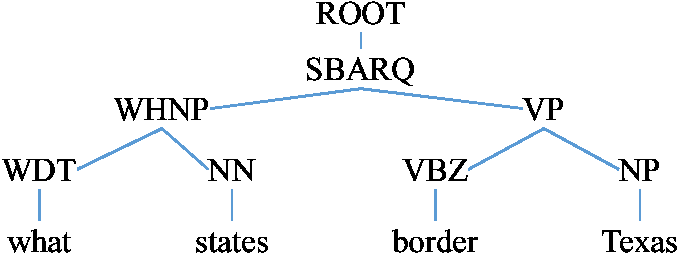
\includegraphics[width=0.48\columnwidth]{figure/rw/qa-parsing-xs.eps}}
  \hspace{1em}
  \subcaptionbox{基于PCCG的语义解析树\cite{zettlemoyer2012learning}\label{fig:rw-spt:b}}
    {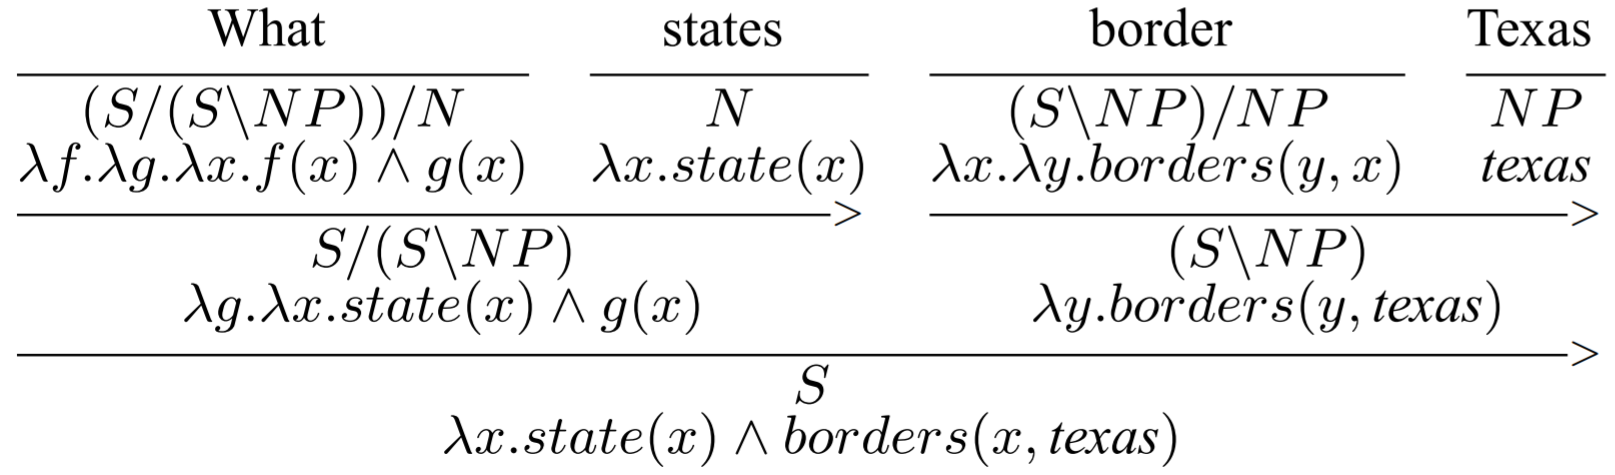
\includegraphics[width=0.48\columnwidth]{figure/rw/qa-ccg-3.png}}

  \vspace{1em}

  \subcaptionbox{基于$\lambda$-DCS的语义解析树\label{fig:rw-spt:c}}
    {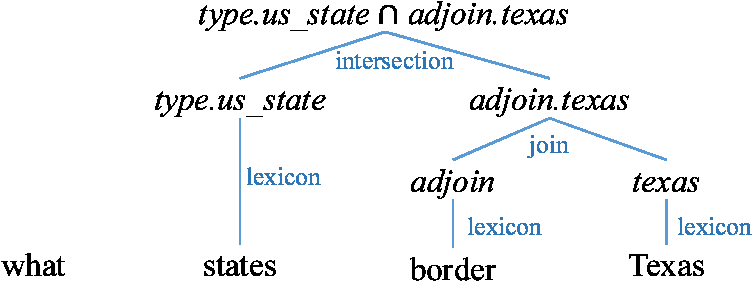
\includegraphics[width=0.48\columnwidth]{figure/rw/qa-dcs-xs.eps}}
  \hspace{3em}
  \subcaptionbox{基于多阶段生成的查询结构\label{fig:rw-spt:d}}
    {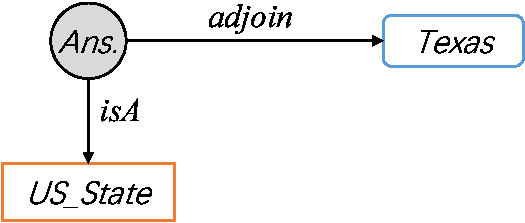
\includegraphics[width=0.38\columnwidth]{figure/rw/qa-stagg-xs.eps}}
  \bicaption{例句 ``what state borders texas'' 的多种解析结构。}
            {Several parsing structures for the question ``what state borders texas''.}
  \label{fig:rw-spt}
\end{figure}

%kwiatkowski2010inducing
%CCG cite
早期的语义解析模型\cite{zettlemoyer2012learning,kwiatkowski2010inducing,cai2013large}
使用概率化组合文法  (Probabilistic Combinatory Categorial Grammar,PCCG)
生成语义解析树。
该方法与语法解析中的概率化上下文无关文法(Probabilistic Context-Free Grammar,PCFG)相似,
根据训练数据学习文法中不同生成式规则的概率值,
并自底向上推理出每个句子最可能生成的成分解析树(Constituency Parsing Tree)。
\figref{fig:rw-spt:a}为例句的成分解析树,描述了整句的语法结构,
并标出了不同短语在句中的成分。
通过PCCG生成的语义解析树如\figref{fig:rw-spt:b}所示,
PCCG的生成式规则中不仅具有代表语法的成分信息,
同时还包含代表语义的$\lambda$表达式,
因此不同成分按照语法规则组合的过程中,
各自$\lambda$表达式也在进行拼接,从而得到对应整句话语义的逻辑表示。
PCCG语法具有很强的语义表示能力,
但由于生成式规则中涉及到不同的$\lambda$表达式,
同时训练数据匮乏,使得模型的训练具有难度。

% CCG: 语法以及语义,用lambda表达式来描述,
% 例如Inducing Probabilistic CCG Grammars from Logical Form
% with Higher-Order Unification
% 的例子,borders的那个
% 不仅语法组合成更高级的结构,语义也具有lambda表达式中的传参
% 
% PCCG: 同样概率介入,因为有多种合并方式。
% (lexicon怎么建,还要涉及词组)
% 特点:完全自底向上,每一个词都有用处(但是不是把问题搞复杂了)
% 可以支持很多操作,例如max、min、order等语义。
% 以及on-the-fly,语义解析树还需要一步转换,定位到特定的KB。


Liang在2013年提出的$\lambda$-DCS\cite{liang2013lambda}
旨在以更加简单的概念和流程,将问句转换为Freebase上的语义解析树。
如\figref{fig:rw-spt:c}所示,生成过程依然是自底向上模式,
叶节点(单词或词组)对应Freebase中的实体、类型或谓词,
但不再具有显式且复杂的$\lambda$表达式。
$\lambda$-DCS定义了节点组合过程的有限种语义合并方式,
包括连接、交集、并集甚至更加高阶的最值、计数等操作,
使得与PCCG相比,
生成的语义解析树在结构更加简单的同时,
牺牲了一定表达能力,
但对于事实类问题的理解来说依然足够。

Yih等人\cite{yih2015semantic}提出了一种多阶段的语义结构生成方法,
如\figref{fig:rw-spt:d}所示,语义解析树被表示为有向图形式,称为查询图,
图中的每一条边以及连接的两个节点,都对应\eqnref{eqn:logic-form}中的三元组。
与之前两种方法的自底向上生成不同,
多阶段语义结构生成基于由简到繁,逐步生成查询图的思路。
最简单的查询图为答案节点通过谓词(或多个谓词构成的序列)连接至
问句中的某一实体,形成仅有一条有向路径构成的查询图。
问句中抽取的其它实体、类型、时间等信息,则通过多个不同的阶段,
逐步连接至已有的路径上,构成更加复杂的查询图。
该方法不受限与问句中词的先后顺序,查询图的生成更加灵活,
在多个问答数据集上均有良好的效果。

Cui等人\cite{cui2017kbqa}提出了一种基于模板的方式,
对问句生成谓词序列形式的语义结构。
模板是对问句抽象表示,它将问句中的实体替换成类型,指代了一组具有相同语法和语义描述的问句,
``what states border \textit{\$location}'' 是一个具体的模板例子。
模板的提取依靠外部的大规模问答数据,
作者对Yahoo! Answers中大约41M问答对进行实体与答案识别后,
生成了约27M不同的模板,并通过EM算法学习其指向谓词序列的条件概率。
对于每一个问句的语义结构生成,则通过生成模型,由模板进行过渡得到不同谓词序列的概率。
这样的方法,优点在于利用大量外部数据获取准确率高的模板以及和语义的匹配,
但模型的召回率可能成为短板,当问句语法不规范时,简单的模板匹配容易失效。
%此外,其它的语义解析结构的生成方式,
%例如基于固定模板的结构生成\parencite{bast2015more,cui2017kbqa},
此外,一些文献\parencite{reddy2016transforming,hu2018answering}
使用了基于依存语法树转换的方式,利用结构相似性实现语义解析结构的生成,
这里不再一一介绍。


\subsubsection{语义匹配模型构建}    %文字1页,图0.25-0.5

由于自然语言的多义性,语义解析结构的生成结果通常都不唯一,
%因此模型需要计算问句与语义结构之间的匹配度,并根据问答数据进行训练。
%排名问题
因此需要对\textless 问句,语义解析结构 \textgreater 的匹配度进行建模,
选择最高匹配度的解析结构进行知识库上的答案查询。
%就三段,别多了
传统的语义解析模型主要基于特征工程,
Berant等人\cite{berant2013semantic}的研究工作为一个典型例子。
语义解析树由$\lambda$-DCS生成,
抽取出的特征包含三类:
问句中的短语与对应知识库谓词的对齐特征,
不同谓词参与合并的特征,
以及解析树的总体结构特征。
前两类特征来自于解析树的自底向上生成过程,用于捕捉每一个操作,
后一类特征则统计解析树中不同类型操作的数量,以及最终返回的答案数量。
%Kwai Cai Berant Bast
%基于特征工程的模型将解析树的生成看做操作序列,

为了弥补特征工程耗费人力的缺陷,同时获取更高层面的语义匹配信号,
Berant等人在后续的工作\parencite{berant2014semantic}中引入了转述特征(Paraphrasing Feature),
通过简单的规则将解析树翻译成自然语言问句,
并衡量原问句和生成问句之间是否具有转述关系,将其作为额外一组特征。
转述关系涉及到自然语言文本匹配问题,
作者使用基于词对应的关联模型和词向量的维度空间模型两种方式进行建模,
使得问答系统可以得到解析树的整体语义,是传统特征工程的有力补充。

最新的自动问答模型广泛使用了深度学习技术。
相关研究的共同点在于遵循一种 ``{编码—比较}'' 框架,
其重点在于,通过神经网络的特征学习能力,
对问句和解析结构分别进行编码,得到各自向量表示,
最后计算向量之间的相似度,代表问句与解析结构的匹配程度。
以简单问题数据集SimpQuestions为代表的问答模型几乎完全属于这一范畴,
由于在SimpleQuestions中,问句的语义解析结构均为单一谓词序列,
因此这些模型本质上都是对文本序列和谓词序列之间的匹配进行建模。
Yu等人\cite{yu2017improved}提出的HR-BiLSTM模型利用循环神经网络进行建模,
如\figref{fig:rw-siamese:a}所示,
谓词序列输入分为两个粒度:以唯一编号表示的编号序列,以及将谓词名称相连的单词序列,
分别通过双向LSTM层进行编码,
问句文本的编码也利用了双向LSTM层,并使用多层间的残差连接方式进行编码,
旨在让模型能同时捕捉单词粒度和问句整体粒度的语义信号。
SimpleQuestions上的其它类似模型还包括
文献\parencite{lukovnikov2017neural,yin2016simple,golub2016character,qu2018question}。

\begin{figure}[ht]
\centering
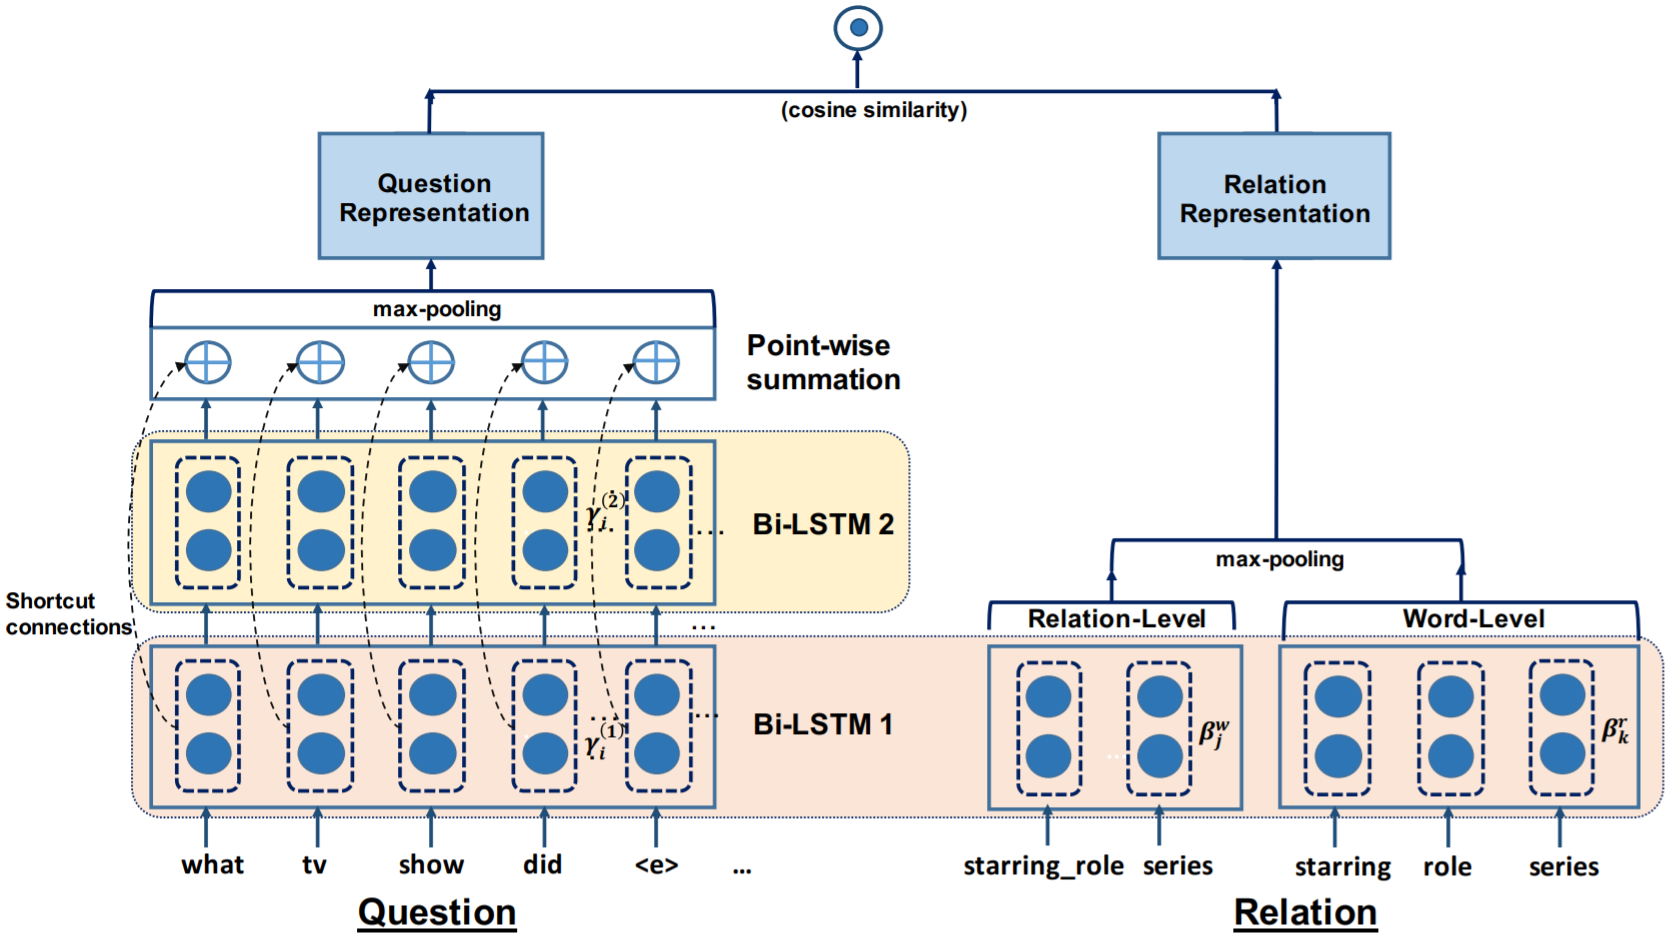
\includegraphics[width=0.95\columnwidth]{figure/rw/qa-hrbilstm.png}
\bicaption{HR-BiLSTM模型。\cite{yu2017improved}}{The HR-BiLSTM model.}
\label{fig:rw-siamese:a}
\end{figure}

对于WebQuestions等数据集上的复杂问题,如同\figref{fig:rw-spt:d}的查询图,
虽包含多条路径,但也可以选择其中最重要的路径作为主体与问句计算匹配程度。
微软的两个自动问答的研究工作\parencite{yih2015semantic,bao2016constraint}
利用了基于卷积神经网络的CDSSM匹配模型\cite{shen2014learning},
对问句和谓词路径的特征学习更多关注局部的词序信息,见\figref{fig:rw-siamese:b}。
其中,前一个研究工作由Yih等人\cite{yih2015semantic}提出,
深度学习模型仅关注问句和最重要谓词路径的匹配度,
对于查询图的其它分支路径,依然使用特征工程的方式寻找问句和谓词的字面匹配。
Bao等人\cite{bao2016constraint}的改进在于同样利用CDSSM模型,
对分支路径与问句中的特定上下文进行匹配,替代了繁琐的特征工程。
然而这些模型并没有能够学习到查询图整体在连续语义空间的特征表达,
不同路径的语义互相独立,因此面对复杂问题仍存在缺陷,这也是我们的研究重点。
%xu的先不聊
%找机会聊Hu和Cui,这两个最好还是提一提

\begin{figure}[ht]
\centering
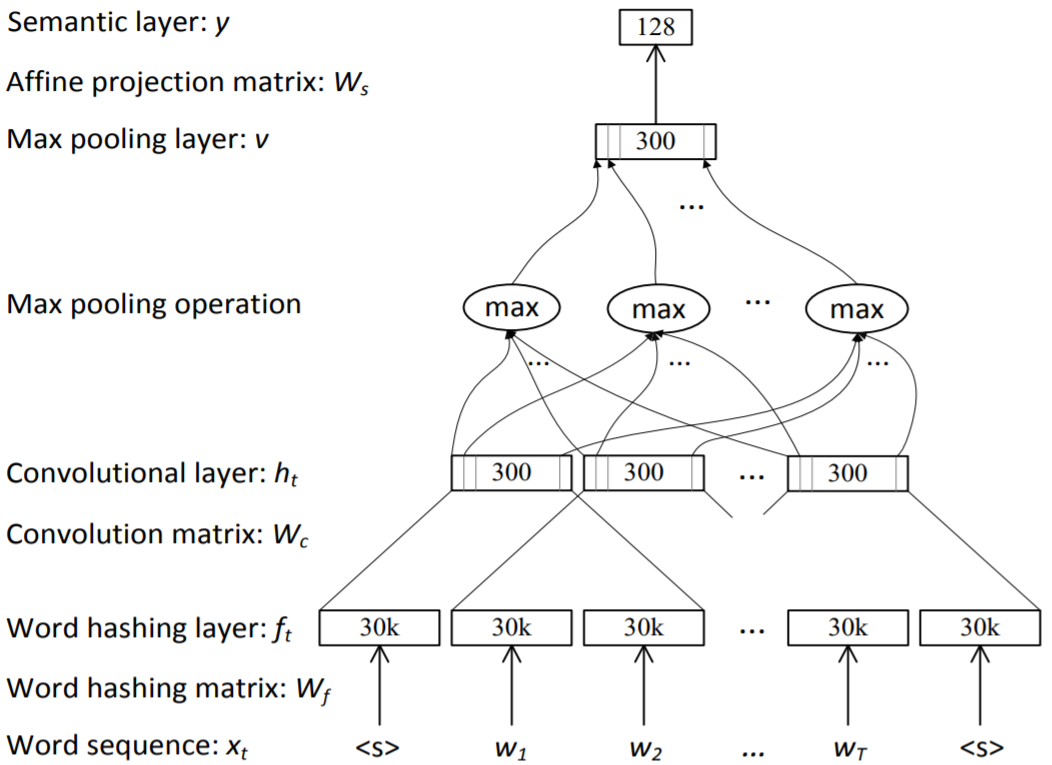
\includegraphics[width=0.6\columnwidth]{figure/rw/qa-cdssm.png}
\bicaption{CDSSM模型。\cite{shen2014learning}}{The CDSSM model.}
\label{fig:rw-siamese:b}
\end{figure}

%\begin{figure}[ht]
%  \centering
%  \subcaptionbox{HR-BiLSTM模型\cite{yu2017improved}\label{fig:rw-siamese:a}}
%    {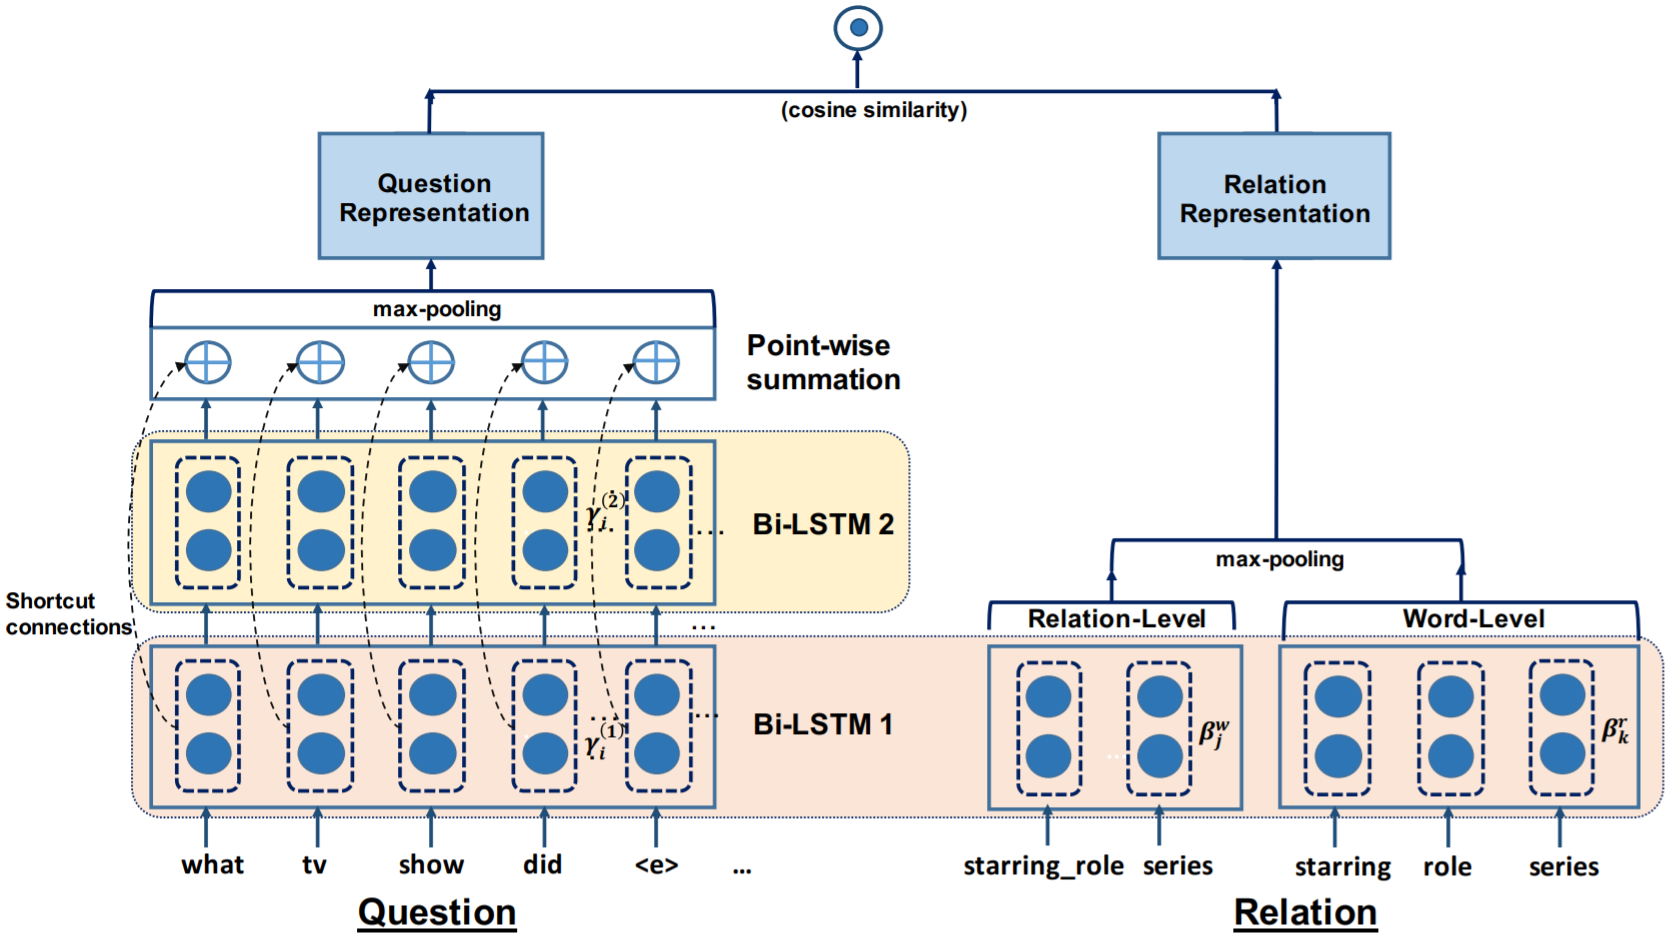
\includegraphics[width=0.48\columnwidth]{figure/rw/qa-hrbilstm.png}}
%  \hspace{1em}
%  \subcaptionbox{CDSSM模型\cite{shen2014learning}\label{fig:rw-siamese:b}}
%    {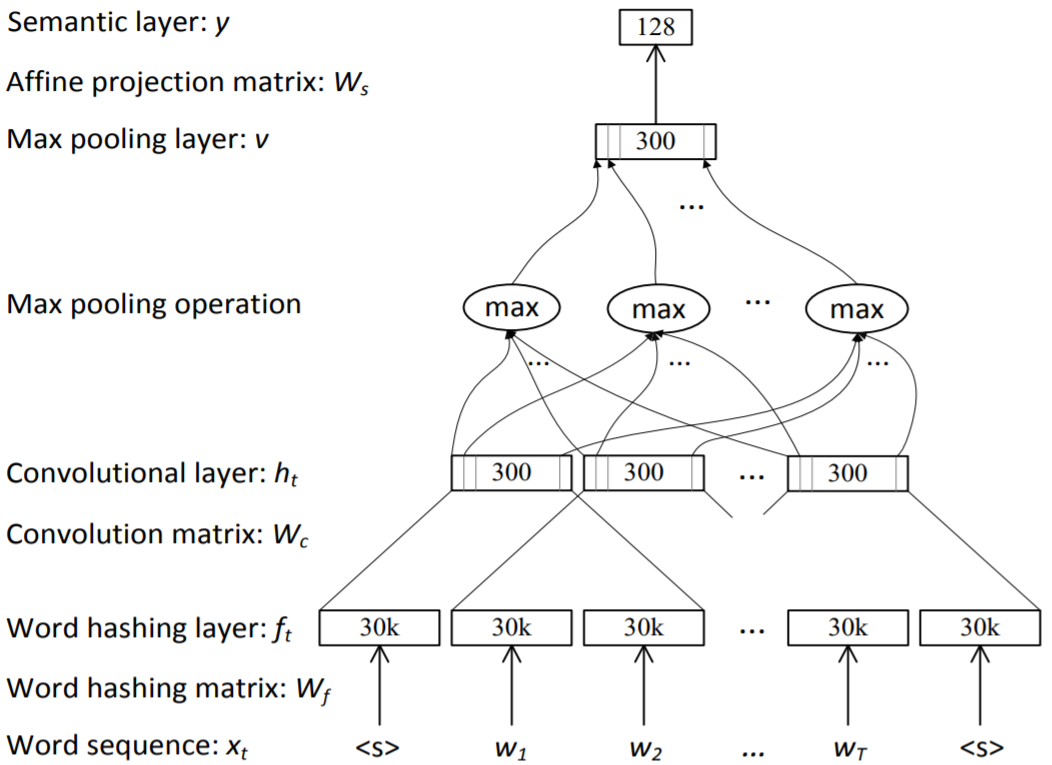
\includegraphics[width=0.48\columnwidth]{figure/rw/qa-cdssm.png}}
%
%  \bicaption{语义解析方法中,用于衡量语义匹配度的神经网络模型示例。}
%            {Example semantic matching models used in semantic parsing approaches.}
%  \label{fig:rw-siamese}
%\end{figure}

\subsubsection{训练方式}

训练方式的不同,主要取决于训练集中是否包含已标注的语义解析结构。
已有的问答数据集中,Free-917人工标注了每个问题的逻辑表达式,
QALD系列数据集则标注了SPARQL查询语句。
对于这些正确结构已给定的数据集,
可以直接利用监督学习算法进行匹配度训练。

显然语义结构的标注需要知识库领域的专家,因此标注过程会消耗大量人力,
更大规模的数据集例如WebQuestions和ComplexQuestions
仅包含每个问题的正确答案,而没有语义结构信息。
对于这些数据集,首先需要通过远距离监督方式构造可直接使用的训练数据,
即对所有训练问题,自动生成语义结构的正负样本。
已有的方法主要利用$F_1$分数衡量语义结构的好坏,
兼顾其生成的查询结果的准确率与召回率,即$F_1=2 \cdot P \cdot R / (P+R)$,
其中$P$代表准确率,$R$代表召回率。
再通过设定阈值将不同的语义结构划分为正负样本,
例如Berant等人\cite{berant2013semantic}仅将$F_1$分值为1(即答案完全匹配)
的语义结构作为正样本,
而Yih等人\cite{yih2015semantic}则将阈值设为0.5,
容忍一定程度的答案不完全匹配。
远距离监督方式避免了人工标注大量语义结构,
但考虑到语义偏差的存在,即答案正确的语义结构未必正确,
自动生成的训练数据也会引入一定量的错误。

%写类似p(g|q)之类的玩意儿刻画loss

%1. Template based (Bast, Yahya?)
%
%2. CCG (UBS, Kwai, CaiYates)
%
%3. DCS (Berant)
%
%4. Dependency Parsing Transform (Reddy, Hu)
%
%5. Staged Parsing (Yih, Bao)
%
%
%如何训练?
%
%传统Feature based (1,2,3)
%
%
%Improvements
%Berant14
%Yih
%Bao
%Xu...




\subsection{基于信息抽取的问答模型}

基于信息抽取的自动问答模型旨在直接从知识库中寻找正确答案,
而不尝试对问题进行具体化的语义建模。
模型主要包含三个步骤:
1) 对问句进行实体链接,得到其中包含的相关实体;
2) 在知识库中抽取出这些相关实体周围的其它实体,构成候选答案集合;
3) 计算问句与每一个候选答案的匹配度,以此预测出其中的正确答案实体。
显然模型的关键点在于第三步,即以怎样的特征描述候选答案与问句之间的关联。
在知识库中,一个实体所具有的信息主要包含它的名称、类型、
直接相连的谓词以及周围的其它实体。
这些信息组成了知识库中以该实体为中心的局部图,
不同的信息抽取模型都以这样的局部图作为候选答案实体的输入。
而这些模型的区别,在于特征的选取或学习方式。

Yao等人\cite{yao2014information}提出的模型利用特征工程方式,
将问句特征与候选答案特征进行配对组合,得到大规模的关联特征。
问句侧的特征来源于依存语法树,从中抽取出不同的依存路径,
以及具有强烈语义的词汇(如动词,wh-疑问词)。
答案侧的特征为答案的类型,以及与问句已知实体相连的谓词路径。
通过训练,具有高相关性的配对特征
(例如疑问词``where'' 与答案类型$location$配对)将具有更高的权重。

深度学习同样适用于基于信息抽取的问答模型。
Bordes等人\cite{bordes2014question}提出了QASE模型,
同样基于``{编码—比较}'' 框架,如\figref{fig:rw-ir:a}所示,
问句和候选答案的局部图分别进行编码,
问句的编码信息为每个词的出现次数,
候选答案则通过二进制编码表示答案实体自身、所属类型、相邻的谓词等信息。
模型学习映射矩阵$W$,将各自编码转换为连续空间上的语义向量,
$W$的每一行对应一个元素(词、实体、类型、谓词)的向量表示,
因此该模型实现了词向量和知识库向量的联合建模。

\begin{figure}[ht]
\centering
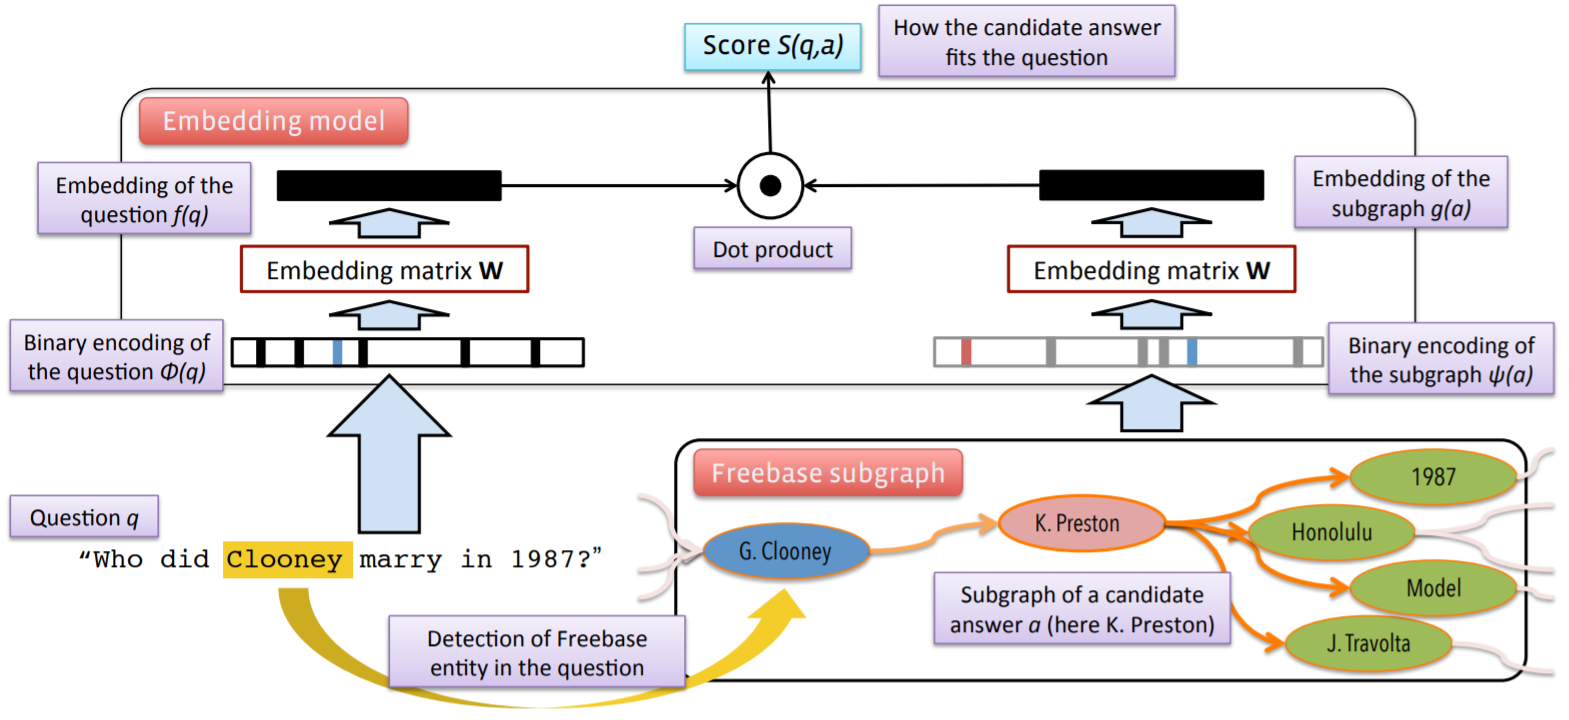
\includegraphics[width=0.95\columnwidth]{figure/rw/qa-qase.png}
\bicaption{QASE模型。\cite{bordes2014question}}{The QASE model.}
\label{fig:rw-ir:a}
\end{figure}

还有一些深度学习模型采用问句分别与答案相关的不同维度信息计算相似度,
再将各个维度的相似度进行聚合,得到问句与候选答案的整体匹配度。
Dong等人\cite{dong2015question}提出了MCCNN模型,
如\figref{fig:rw-ir:b}所示,
模型使用多个不同的卷积神经网络层对问句进行编码,
从而得到问句针对不同信息的向量表达。
将它们分别与答案的类型、谓词、上下文向量表达计算相似度之后,
最终的匹配度为这些相似度分值的总和,
使得模型在寻找最佳答案时能兼顾来自不同方面的匹配特征。

\begin{figure}[ht]
\centering
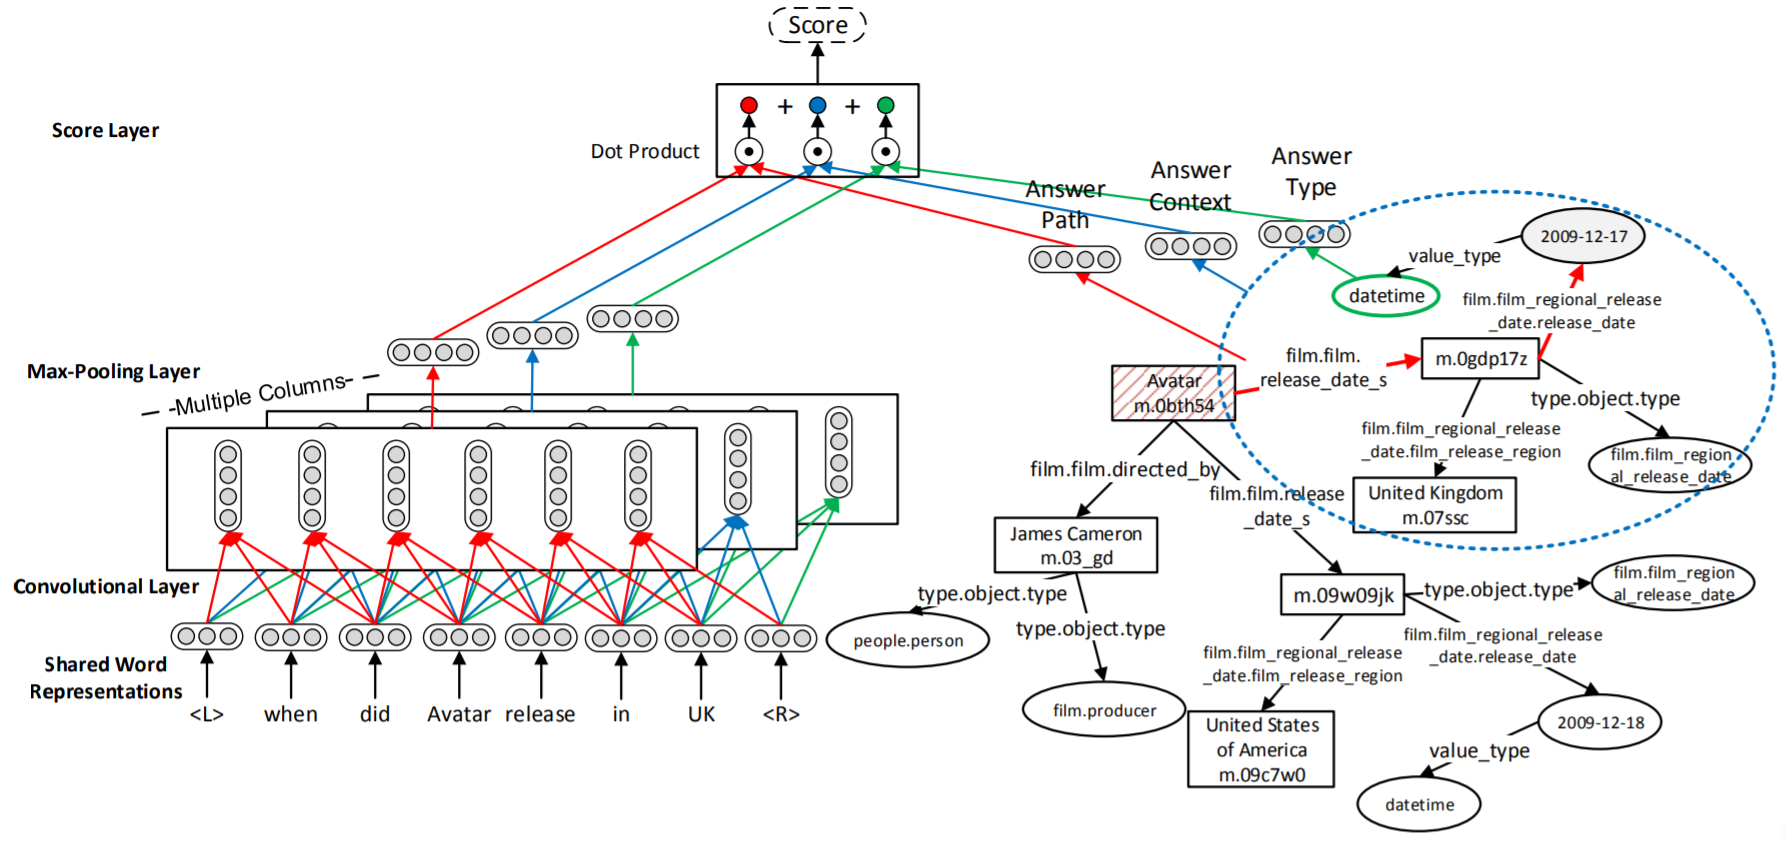
\includegraphics[width=0.95\columnwidth]{figure/rw/qa-mccnn.png}
\bicaption{MCCNN模型。\cite{dong2015question}}{The MCCNN model.}
\label{fig:rw-ir:b}
\end{figure}

Hao等人\cite{hao2017end}的模型在MCCNN基础上进行了改良,
除了将问句编码多个卷积层改为唯一一个双向LSTM层以外,
主要的贡献在于模型中使用了问句和答案之间的双向注意力机制。
一方面,针对答案在不同方面的表达,
答案对问句的注意力能够动态调整问句中不同词的重要性,
另一方面,问句对答案的注意力使得多个相似度分值互相之间也具有权重,
模型训练效果要优于无差别的求和操作。

%\begin{figure}[ht]
%  \centering
%  \subcaptionbox{QASE模型\cite{bordes2014question}\label{fig:rw-ir:a}}
%    {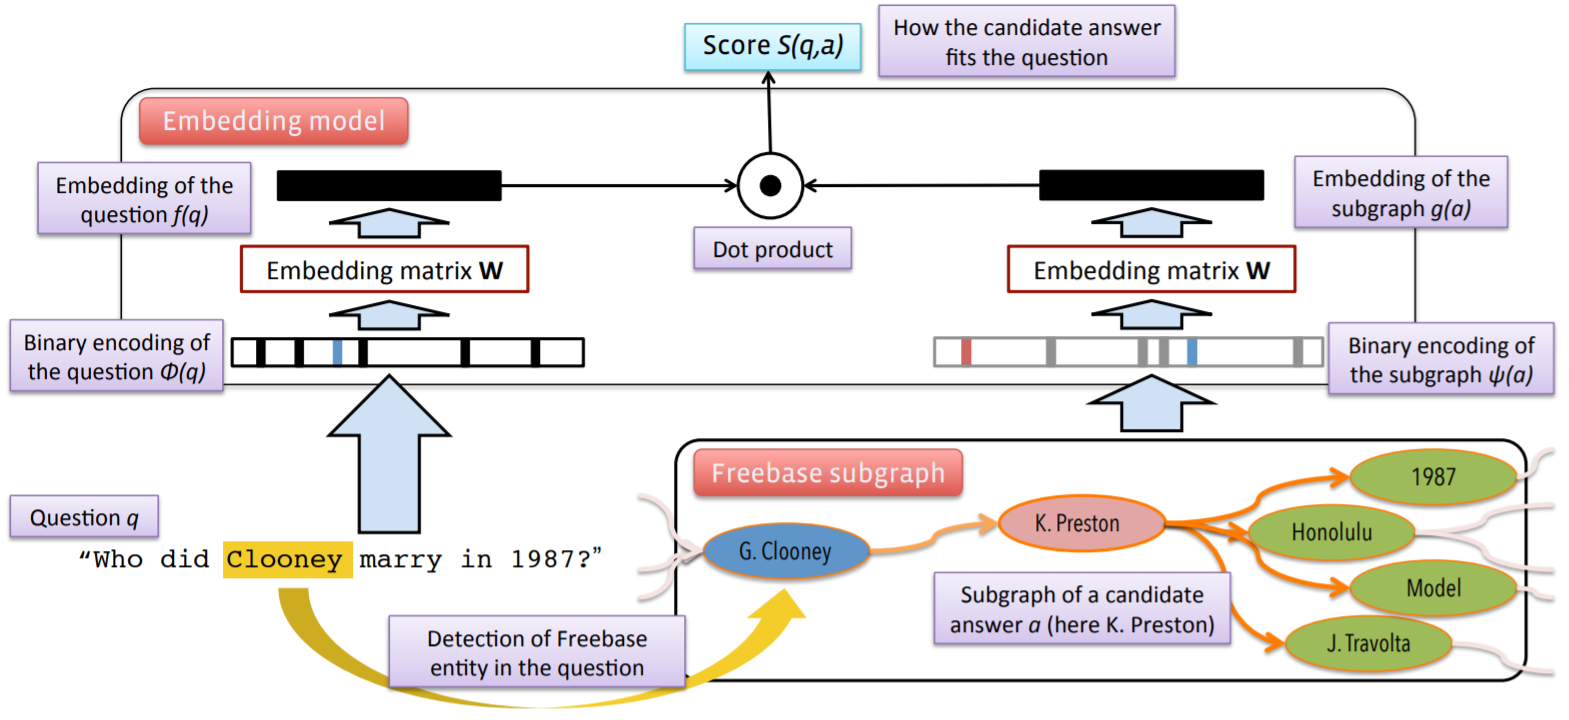
\includegraphics[width=0.48\columnwidth]{figure/rw/qa-qase.png}}
%  \hspace{1em}
%  \subcaptionbox{MCCNN模型\cite{dong2015question}\label{fig:rw-ir:b}}
%    {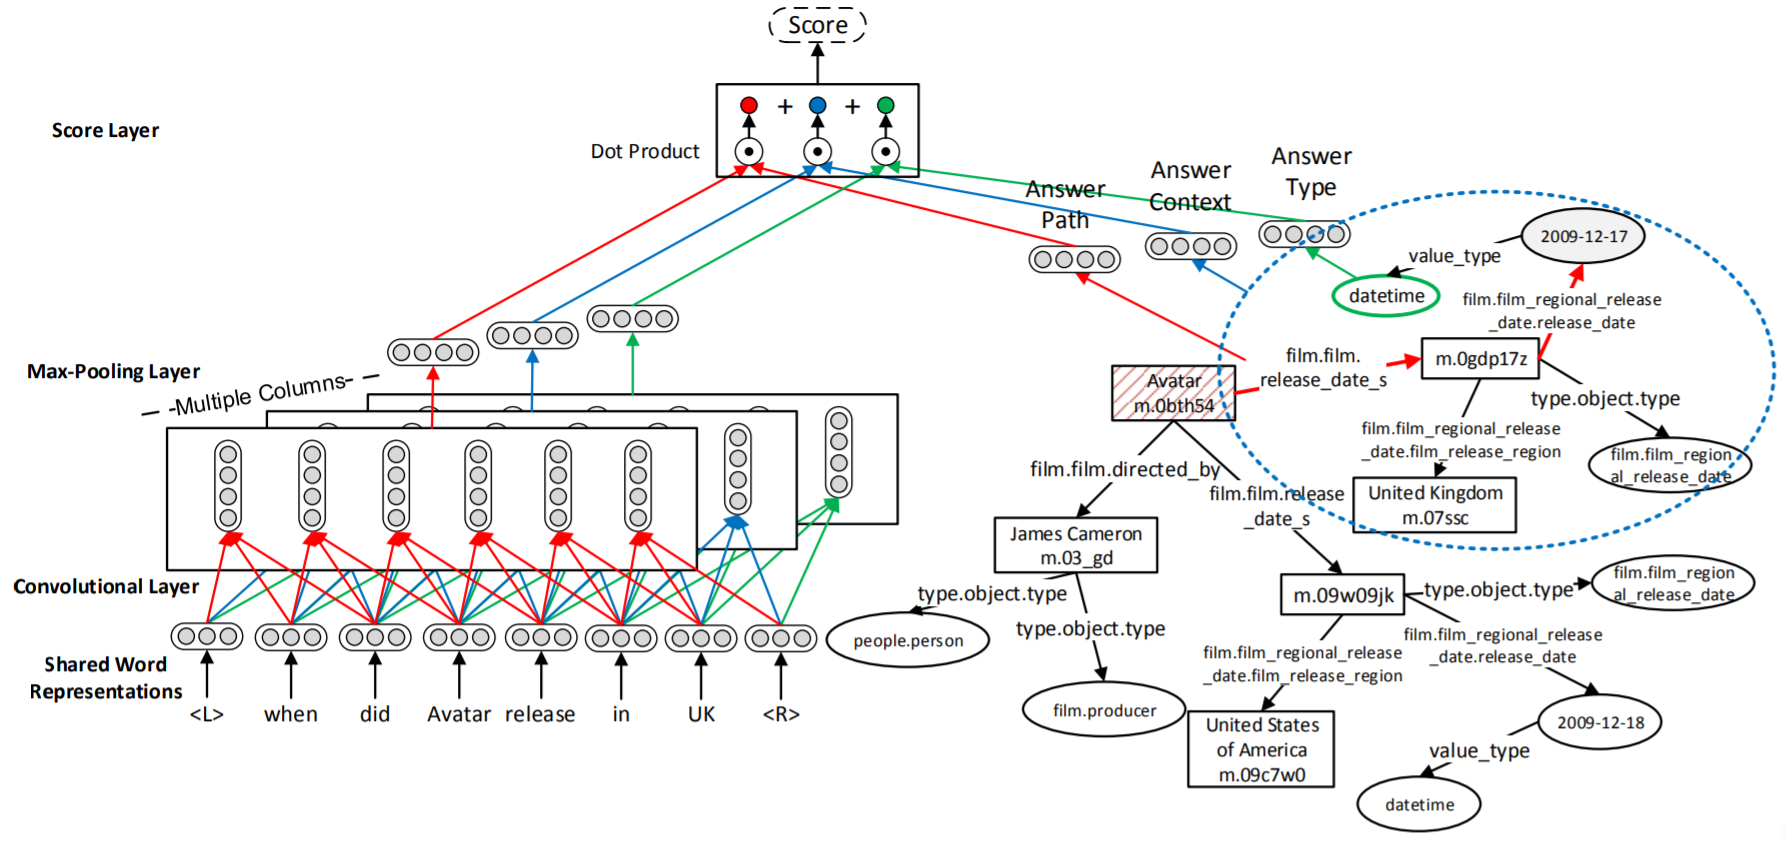
\includegraphics[width=0.48\columnwidth]{figure/rw/qa-mccnn.png}}
%
%  \bicaption{信息抽取方法中,用于衡量语义匹配度的神经网络模型示例。}
%            {Example semantic matching models used in information retrieval approaches.}
%  \label{fig:rw-ir}
%\end{figure}

和语义解析模型比较,
信息抽取模型实现了问答系统的端到端训练,
直接以\textless 问题,答案 \textgreater 作为训练数据,
防止远距离监督引入错误。
但同时也具有解释性较低的缺陷,
无法直接输出模型所理解的问句语义结构,
有时答案预测虽正确,但特征中可能存在语义偏差。
对于复杂语义的自动问答研究,
我们更在意语义结构的正确性,它能直接体现一个问答模型是否具有良好的语义理解能力。


